\documentclass[10pt, onecolumn, draftclsnofoot, letterpaper, compsoc]{IEEEtran}

\usepackage{graphicx}
\usepackage{amssymb}
\usepackage{amsmath}
\usepackage{amsthm}
\usepackage{alltt}
\usepackage{color}
\usepackage{url}
\usepackage{minted}

\graphicspath{ {images/} }

\renewcommand*\contentsname{Table of Contents} % Rename ToC

% Temp title and author
\title{Midterm Progress Report}
\author{Totality AweSun \\
		Bret~Lorimore, Jacob~Fenger, George~Harder \\
		\textit{May 15, 2017 \\
		CS 463 - Spring 2017}}

\begin{document}

\maketitle

\begin{abstract}
This document describes the current state of the \textit{North American Solar Eclipse 2017}
senior capstone project. The document gives a brief overview of the project and its components,
describes the current state of the project, describes problems that have been
encountered throughout the term, shows some of the code that has been produced thus far, gives
a week-by-week outline of progress throughout the term, and reflects over the term in the
retrospectives section at the end.
\end{abstract}

\newpage

\tableofcontents

\newpage

%%%%%%%%%%%%%%%%%%%%%%%%
%   Project Overview   %
%%%%%%%%%%%%%%%%%%%%%%%%
\section{Project Overview}

The North American Solar Eclipse 2017 Senior Capstone project is partnered
with Google to build a set of applications that will assist the development of
the Eclipse Megamovie Project. The overall project has been broken down into
three components: the eclipse image processor, the image processor manager, and
the solar eclipse simulator. Each will be individually outlined in the sections
below. \\

\subsection{Image Processor}

The image processor’s primary activity is to quickly and consistently identify
images of an eclipse at totality. The Eclipse Megamovie project will be
collecting thousands of images from photographers around the country, and the
image processor needs to identify the images of the eclipse at totality so that
these can then be stitched into a timelapse movie. The image processor finds the
sun and moon in each image to determine if it is in a state of totality. The
processor takes in a variety of command line arguments, the only required
one being an images file containing paths to every image to be processed.

In addition to identifying circles in the images, the image processor exports
relevant data, including the processed images, to an output directory. \\

\subsection{Image Processor Developer Pipeline}

\subsection{Eclipse Simulator}

The eclipse simulator will be an independent JavaScript module that can easily
be added to the existing Eclipse Megamovie webpage. This simulator will allow
users to “preview” the eclipse. It will be a 2D depiction of what the solar
eclipse in 2017 could look like given a certain location. Users will be able
to interact with a time slider that will simulate the eclipse in a time
window spanning from 12 hours before the eclipse to 12 hours after it.

To help with the eclipse ephemeris computations, we will be using an external
JavaScript library called MeeusJs. For the front end view for the simulator,
we will be utilizing HTML5 SVG. We plan to implement a model-view-controller
architecture for controlling the states of each component as well as handling
the interactions. This architecture was chosen due to the ability to easily
exchange a component without altering the whole design of the system. For
example, if one wanted to create a whole new front end for the simulator,
they would not need to rewrite the model or controller component of the system.
They would simply need to ensure that the new view component can handle the
interactions with the controller module. \\


%%%%%%%%%%%%%%%%%%%%%%%%
%   Current Status     %
%%%%%%%%%%%%%%%%%%%%%%%%
\section{Current Status of the Project}

Lorem \\

\subsection{Image Processor}

Lorem \\

\subsection{Image Processor Developer Pipeline}

Lorem \\

\subsection{Eclipse Simulator}

Lorem \\


%%%%%%%%%%%%%%%%%%%%%%%%
%   Problems           %
%%%%%%%%%%%%%%%%%%%%%%%%
\section{Problems and Possible Solutions}

We have not come across any problems during Spring term.

%%%%%%%%%%%%%%%%%%%%%%%%
%   Things Left to Do  %
%%%%%%%%%%%%%%%%%%%%%%%%
\section{Things Left to Do}

\subsection{Image Processor}

No further work is needed for the image processor. It successfully ingests
eclipse images, attempts to find the sun/moon, and exports data to an output
directory. Developers who wish to change certain components of the
processor will easily be able to do so. \\

\subsection{Image Processor Developer Pipeline}

None! The pipeline is capable of building and invoking the processor on requested
images. It will then assemble the results into an HTML file which will be uploaded
as well as the processed images to Google Cloud Storage. \\

\subsection{Eclipse Simulator}

None! The simulator is now on the Eclipsemega.movie website and nothing more
is required from us development wise. \\

\subsection{[SUPPLEMENTAL] Eclipse Image Classifier}

We would like to improve the overall accuracy of the classifier as it currently
is only about 70\% accurate. This will potentially require a larger
set of training data which our client is working to gather. \\

%%%%%%%%%%%%%%%%%%%%%%%%
%   Code               %
%%%%%%%%%%%%%%%%%%%%%%%%
\newpage
\section{Interesting Code}

// Code -- image processor?

\begin{minted}{cpp}
int a = b;
\end{minted}

\newpage
\section{Screenshots}

\begin{figure}[!h]
	\begin{center}
  		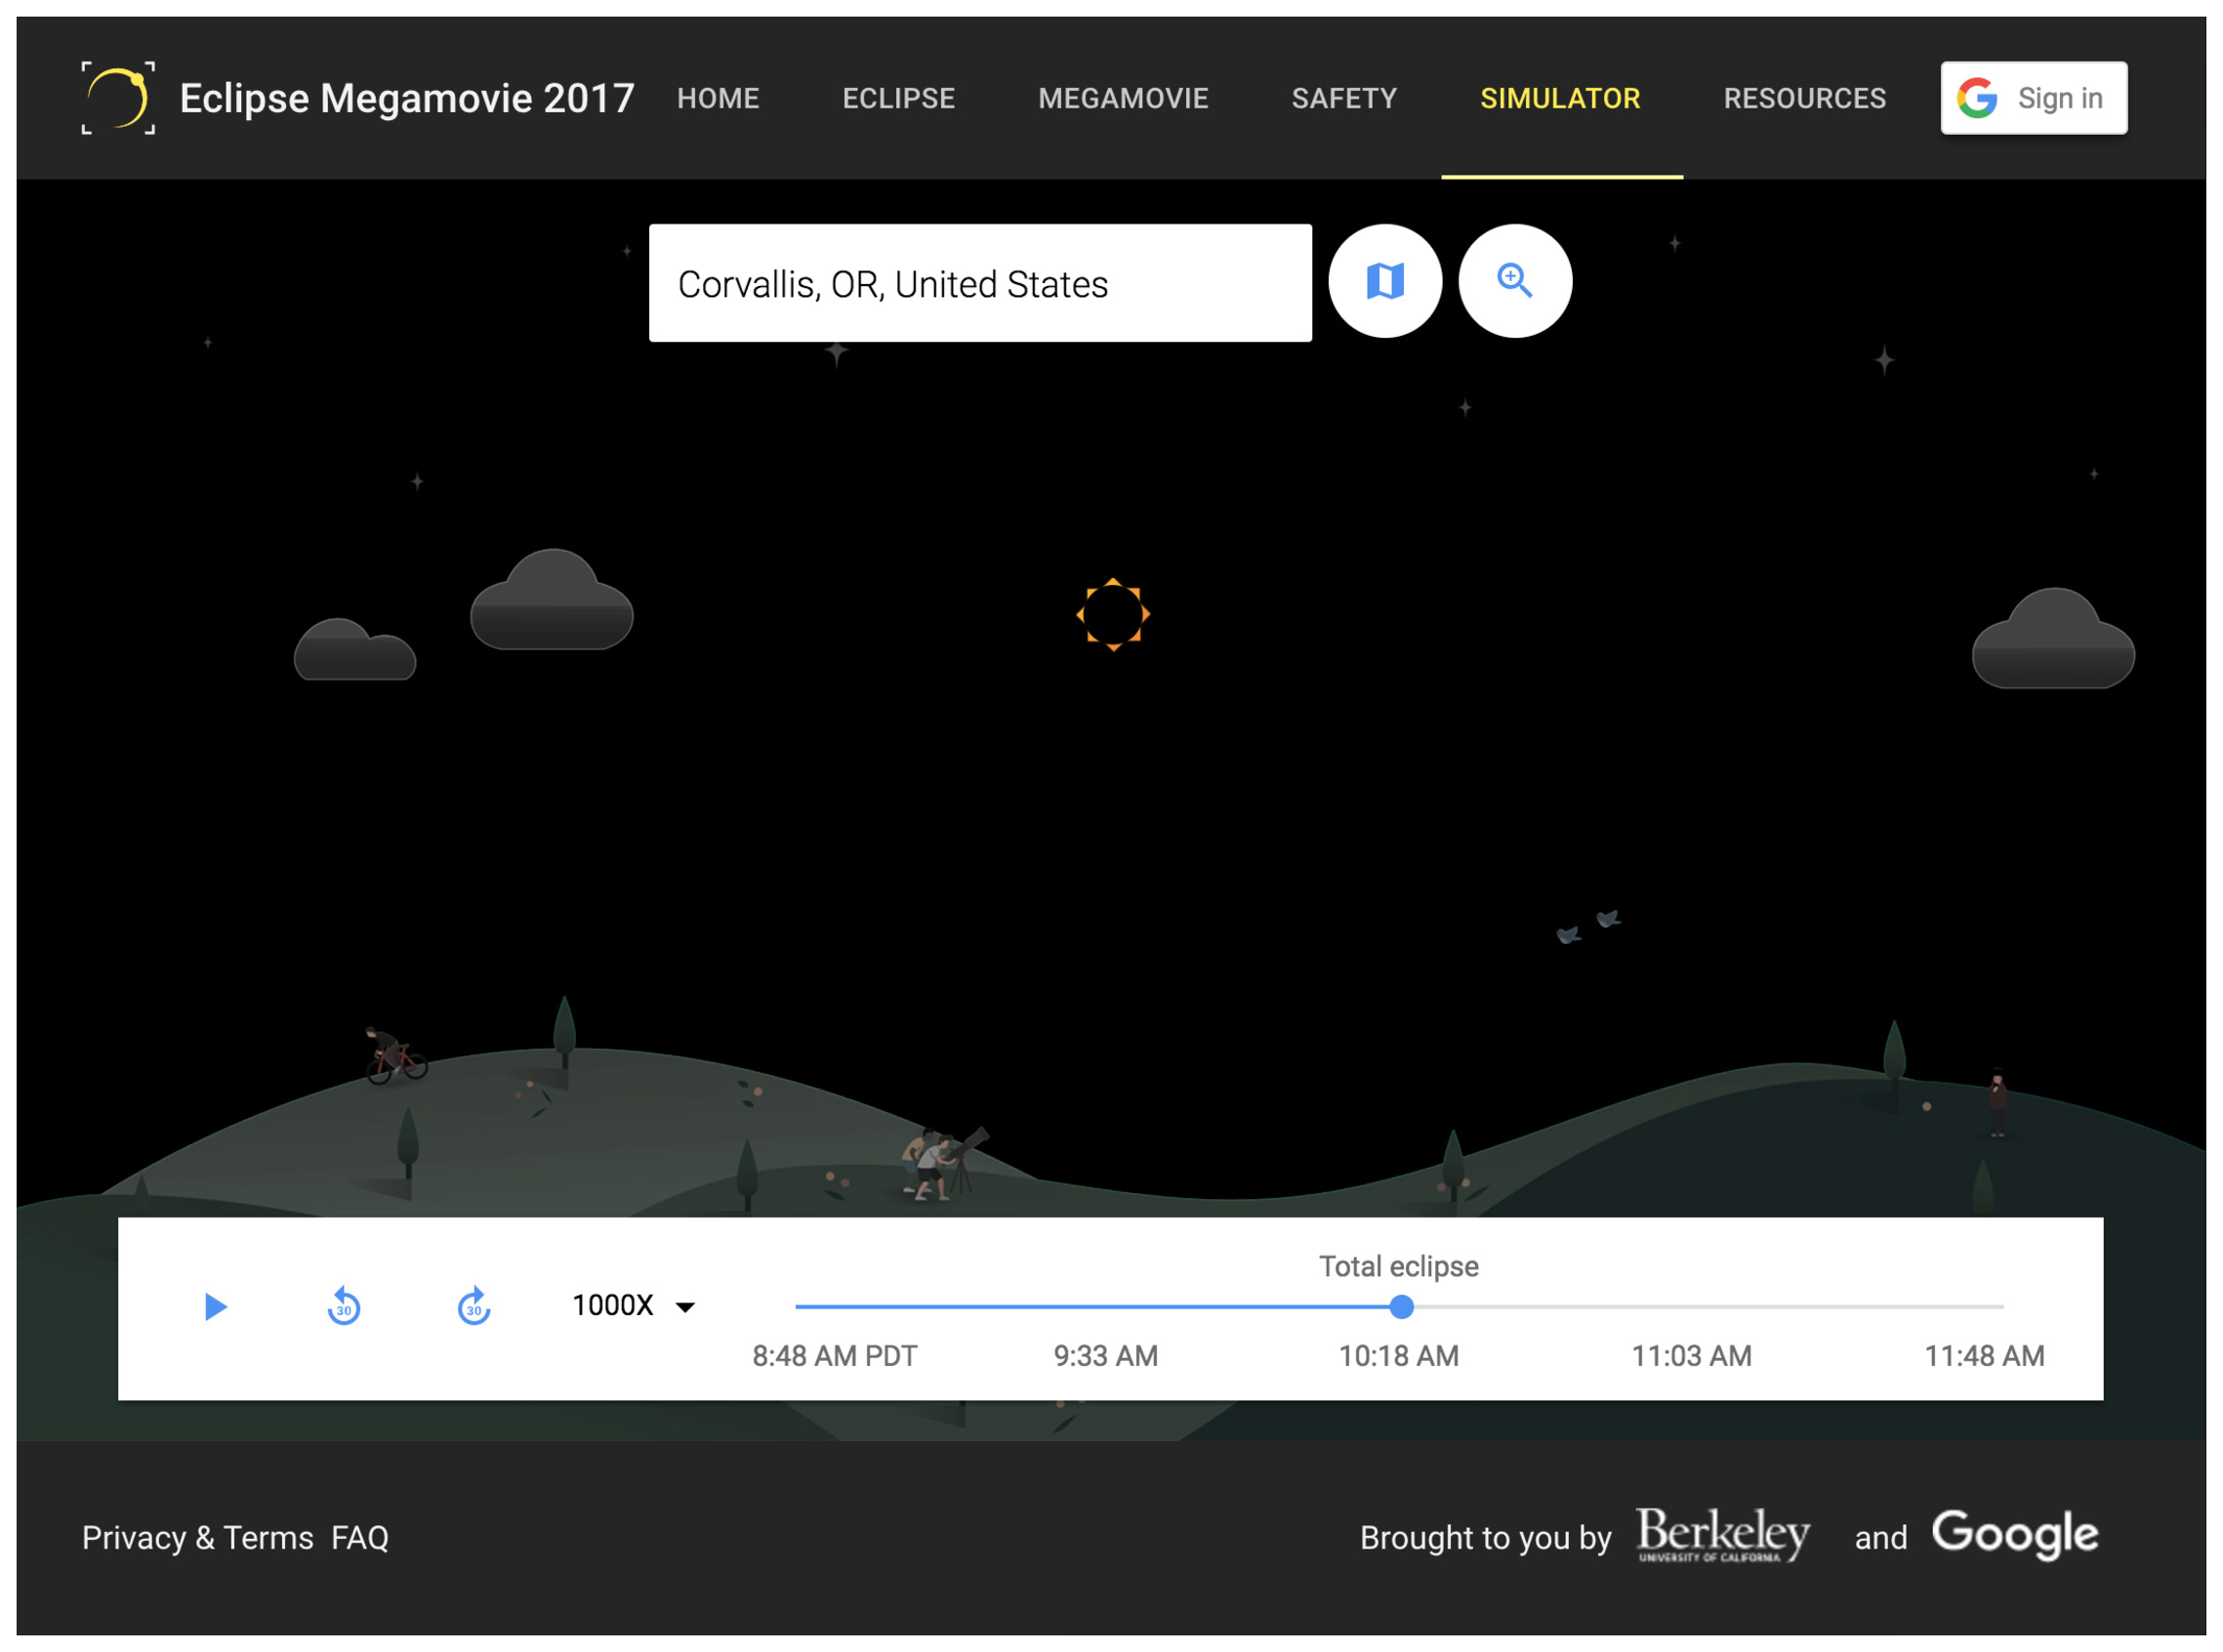
\includegraphics[width=\textwidth]{sim_total.eps}
		\caption{Simulator in wide mode showing a total solar eclipse}
	\end{center}
\end{figure}
\newpage

\begin{figure}[!h]
	\begin{center}
			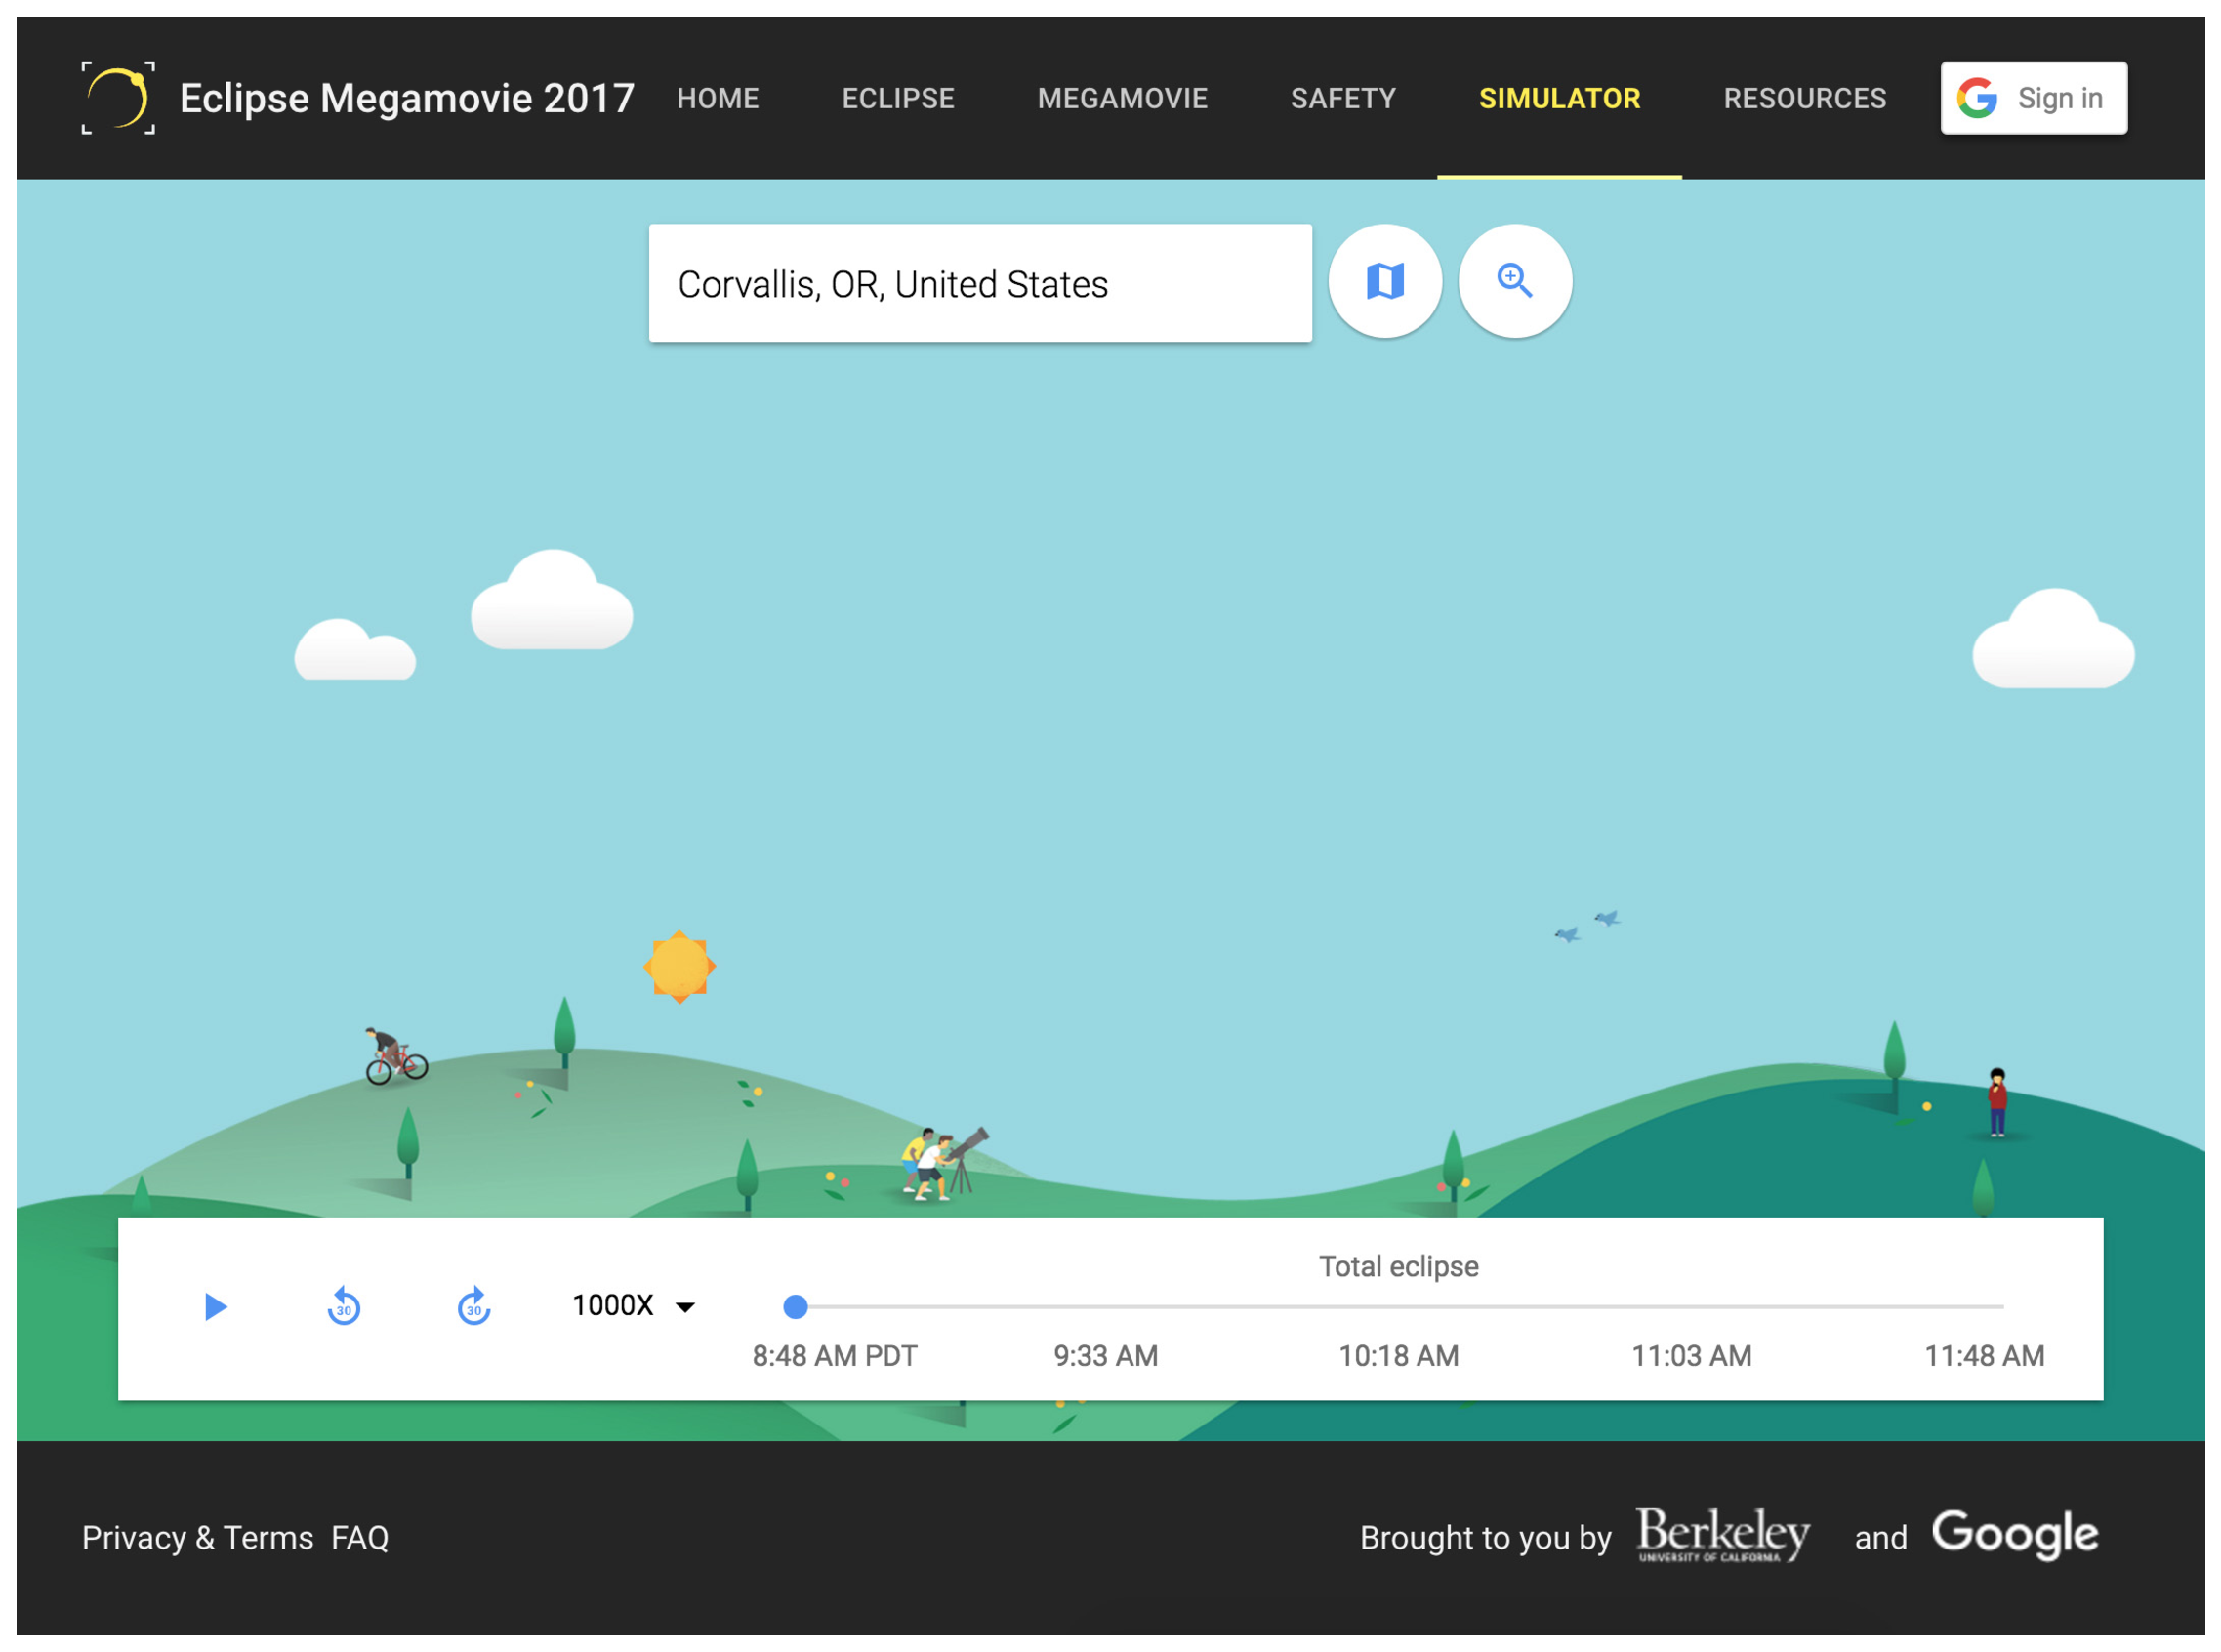
\includegraphics[width=\textwidth]{sim.eps}
		\caption{Simulator in wide mode showing no eclipse}
	\end{center}
\end{figure}
\newpage

\begin{figure}[!h]
	\begin{center}
			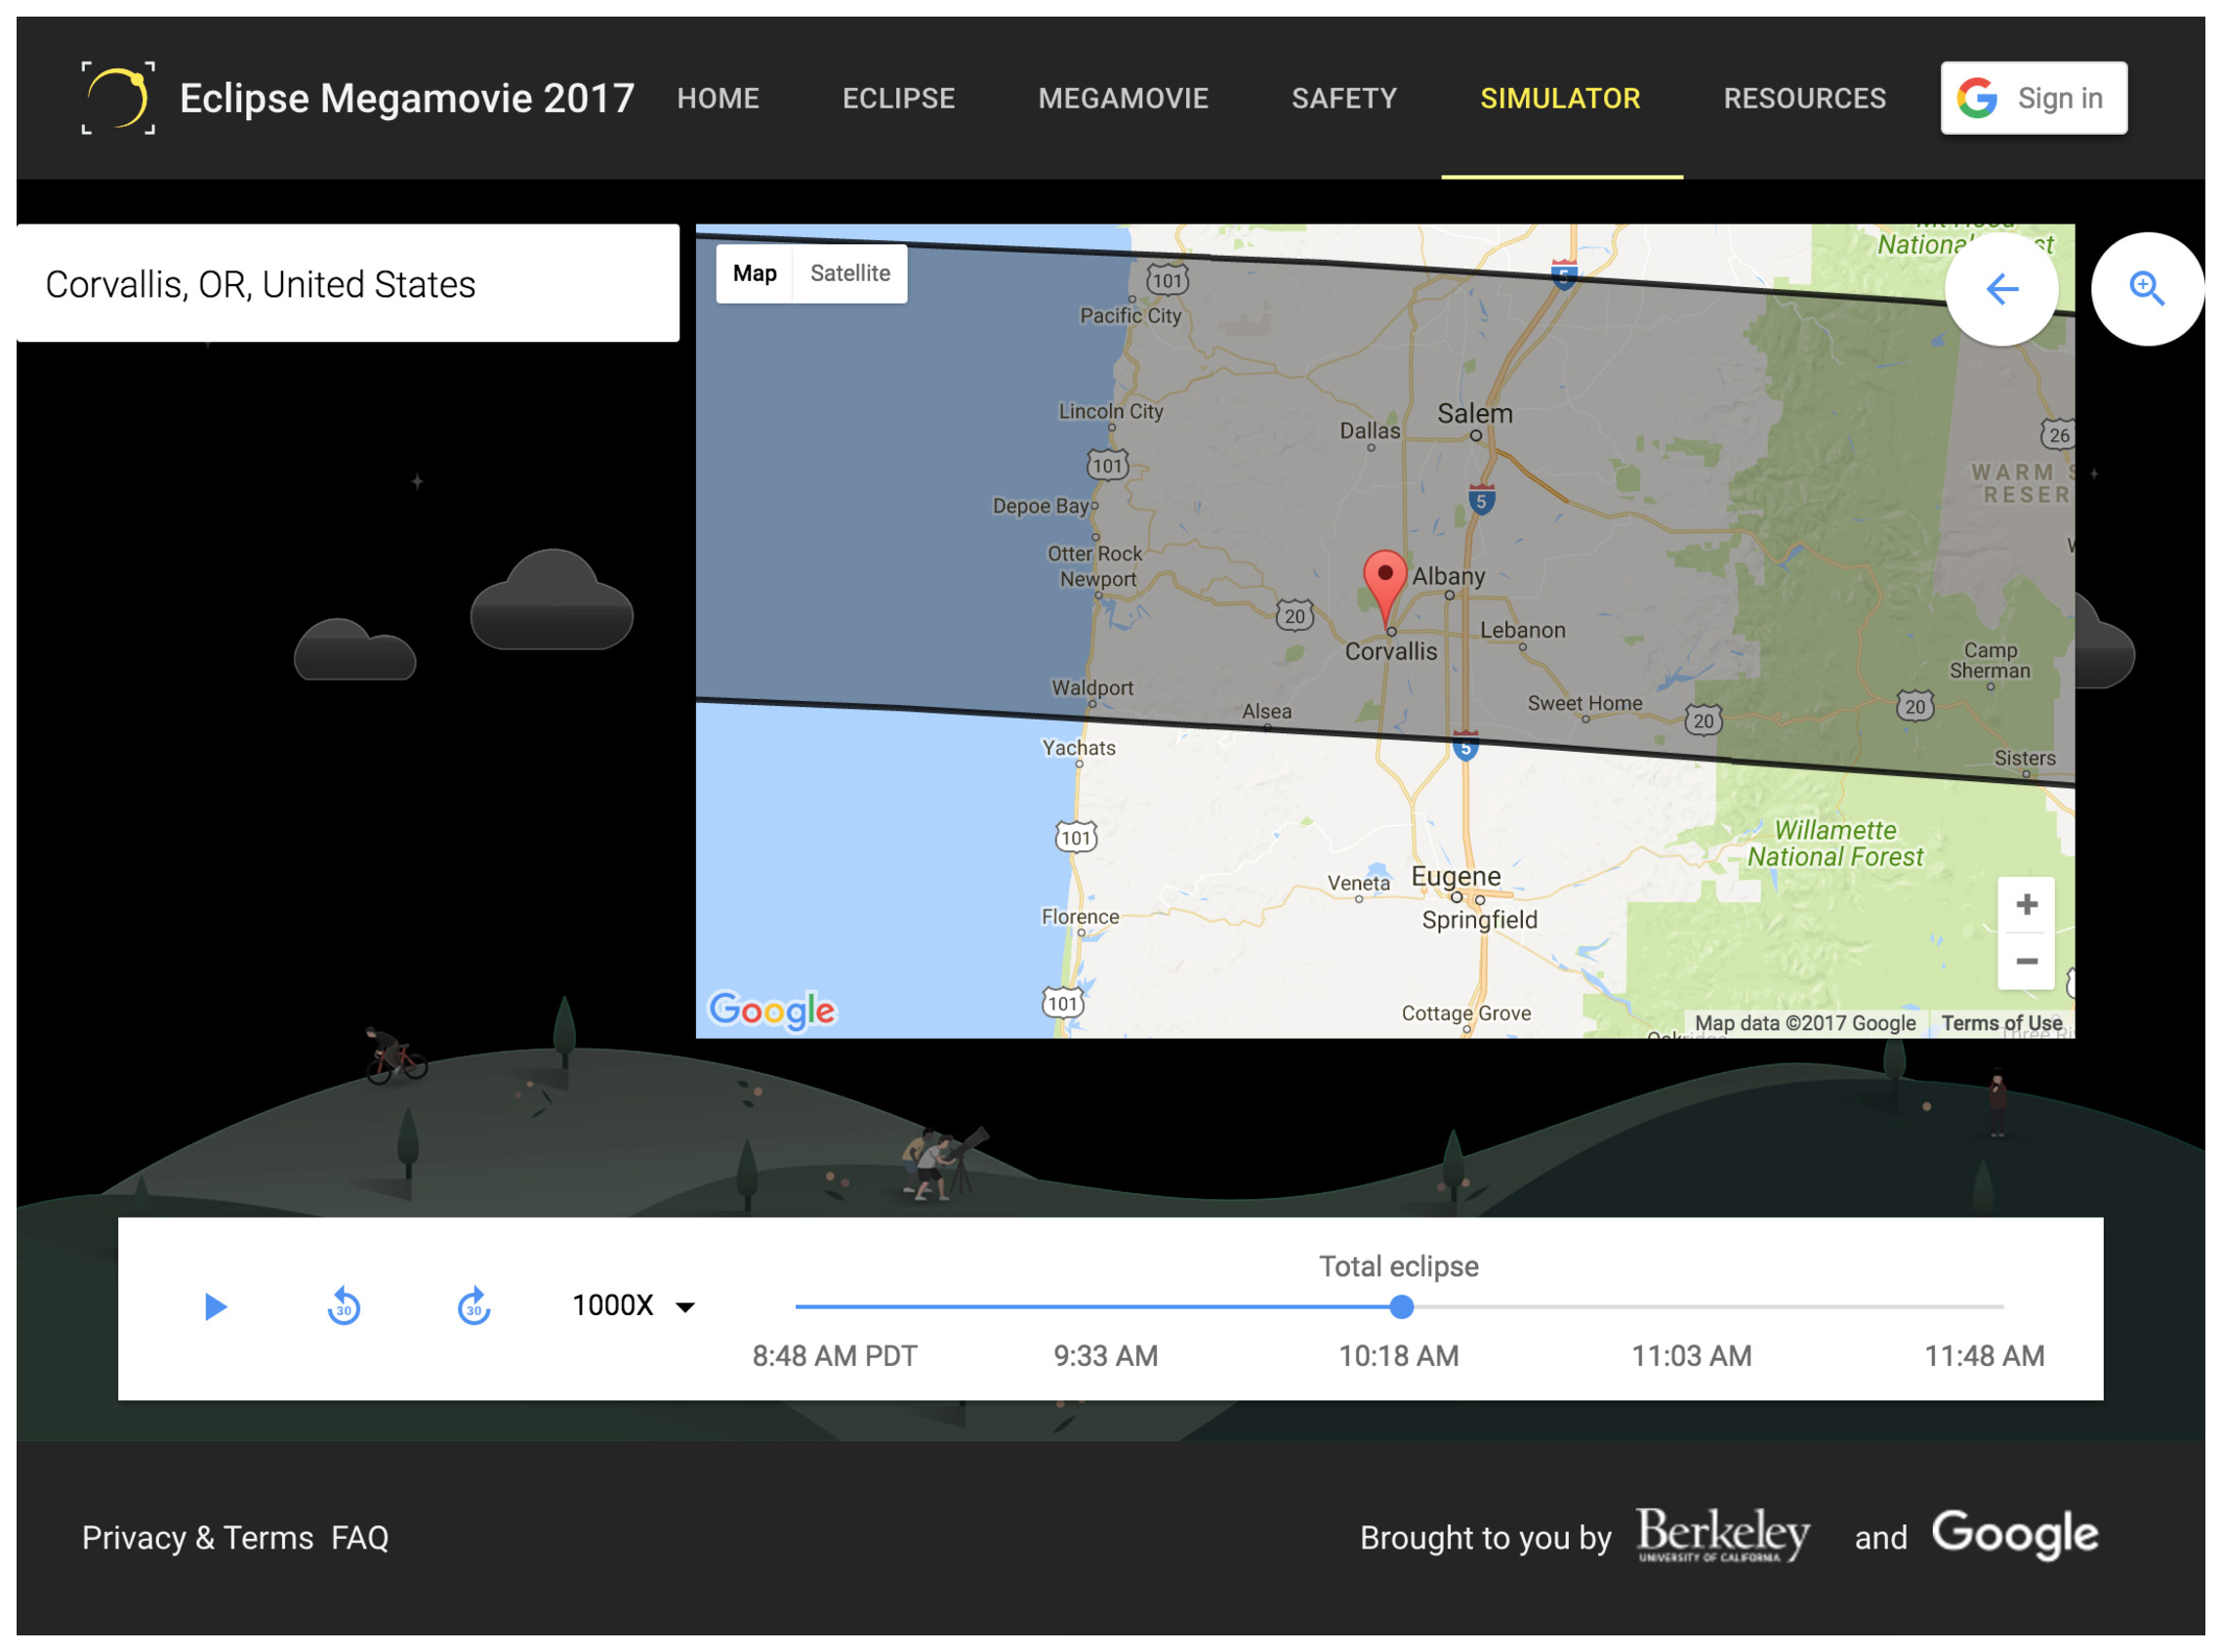
\includegraphics[width=\textwidth]{sim_map.eps}
		\caption{Simulator with map expanded}
	\end{center}
\end{figure}
\newpage

\begin{figure}[!h]
    \begin{center}
            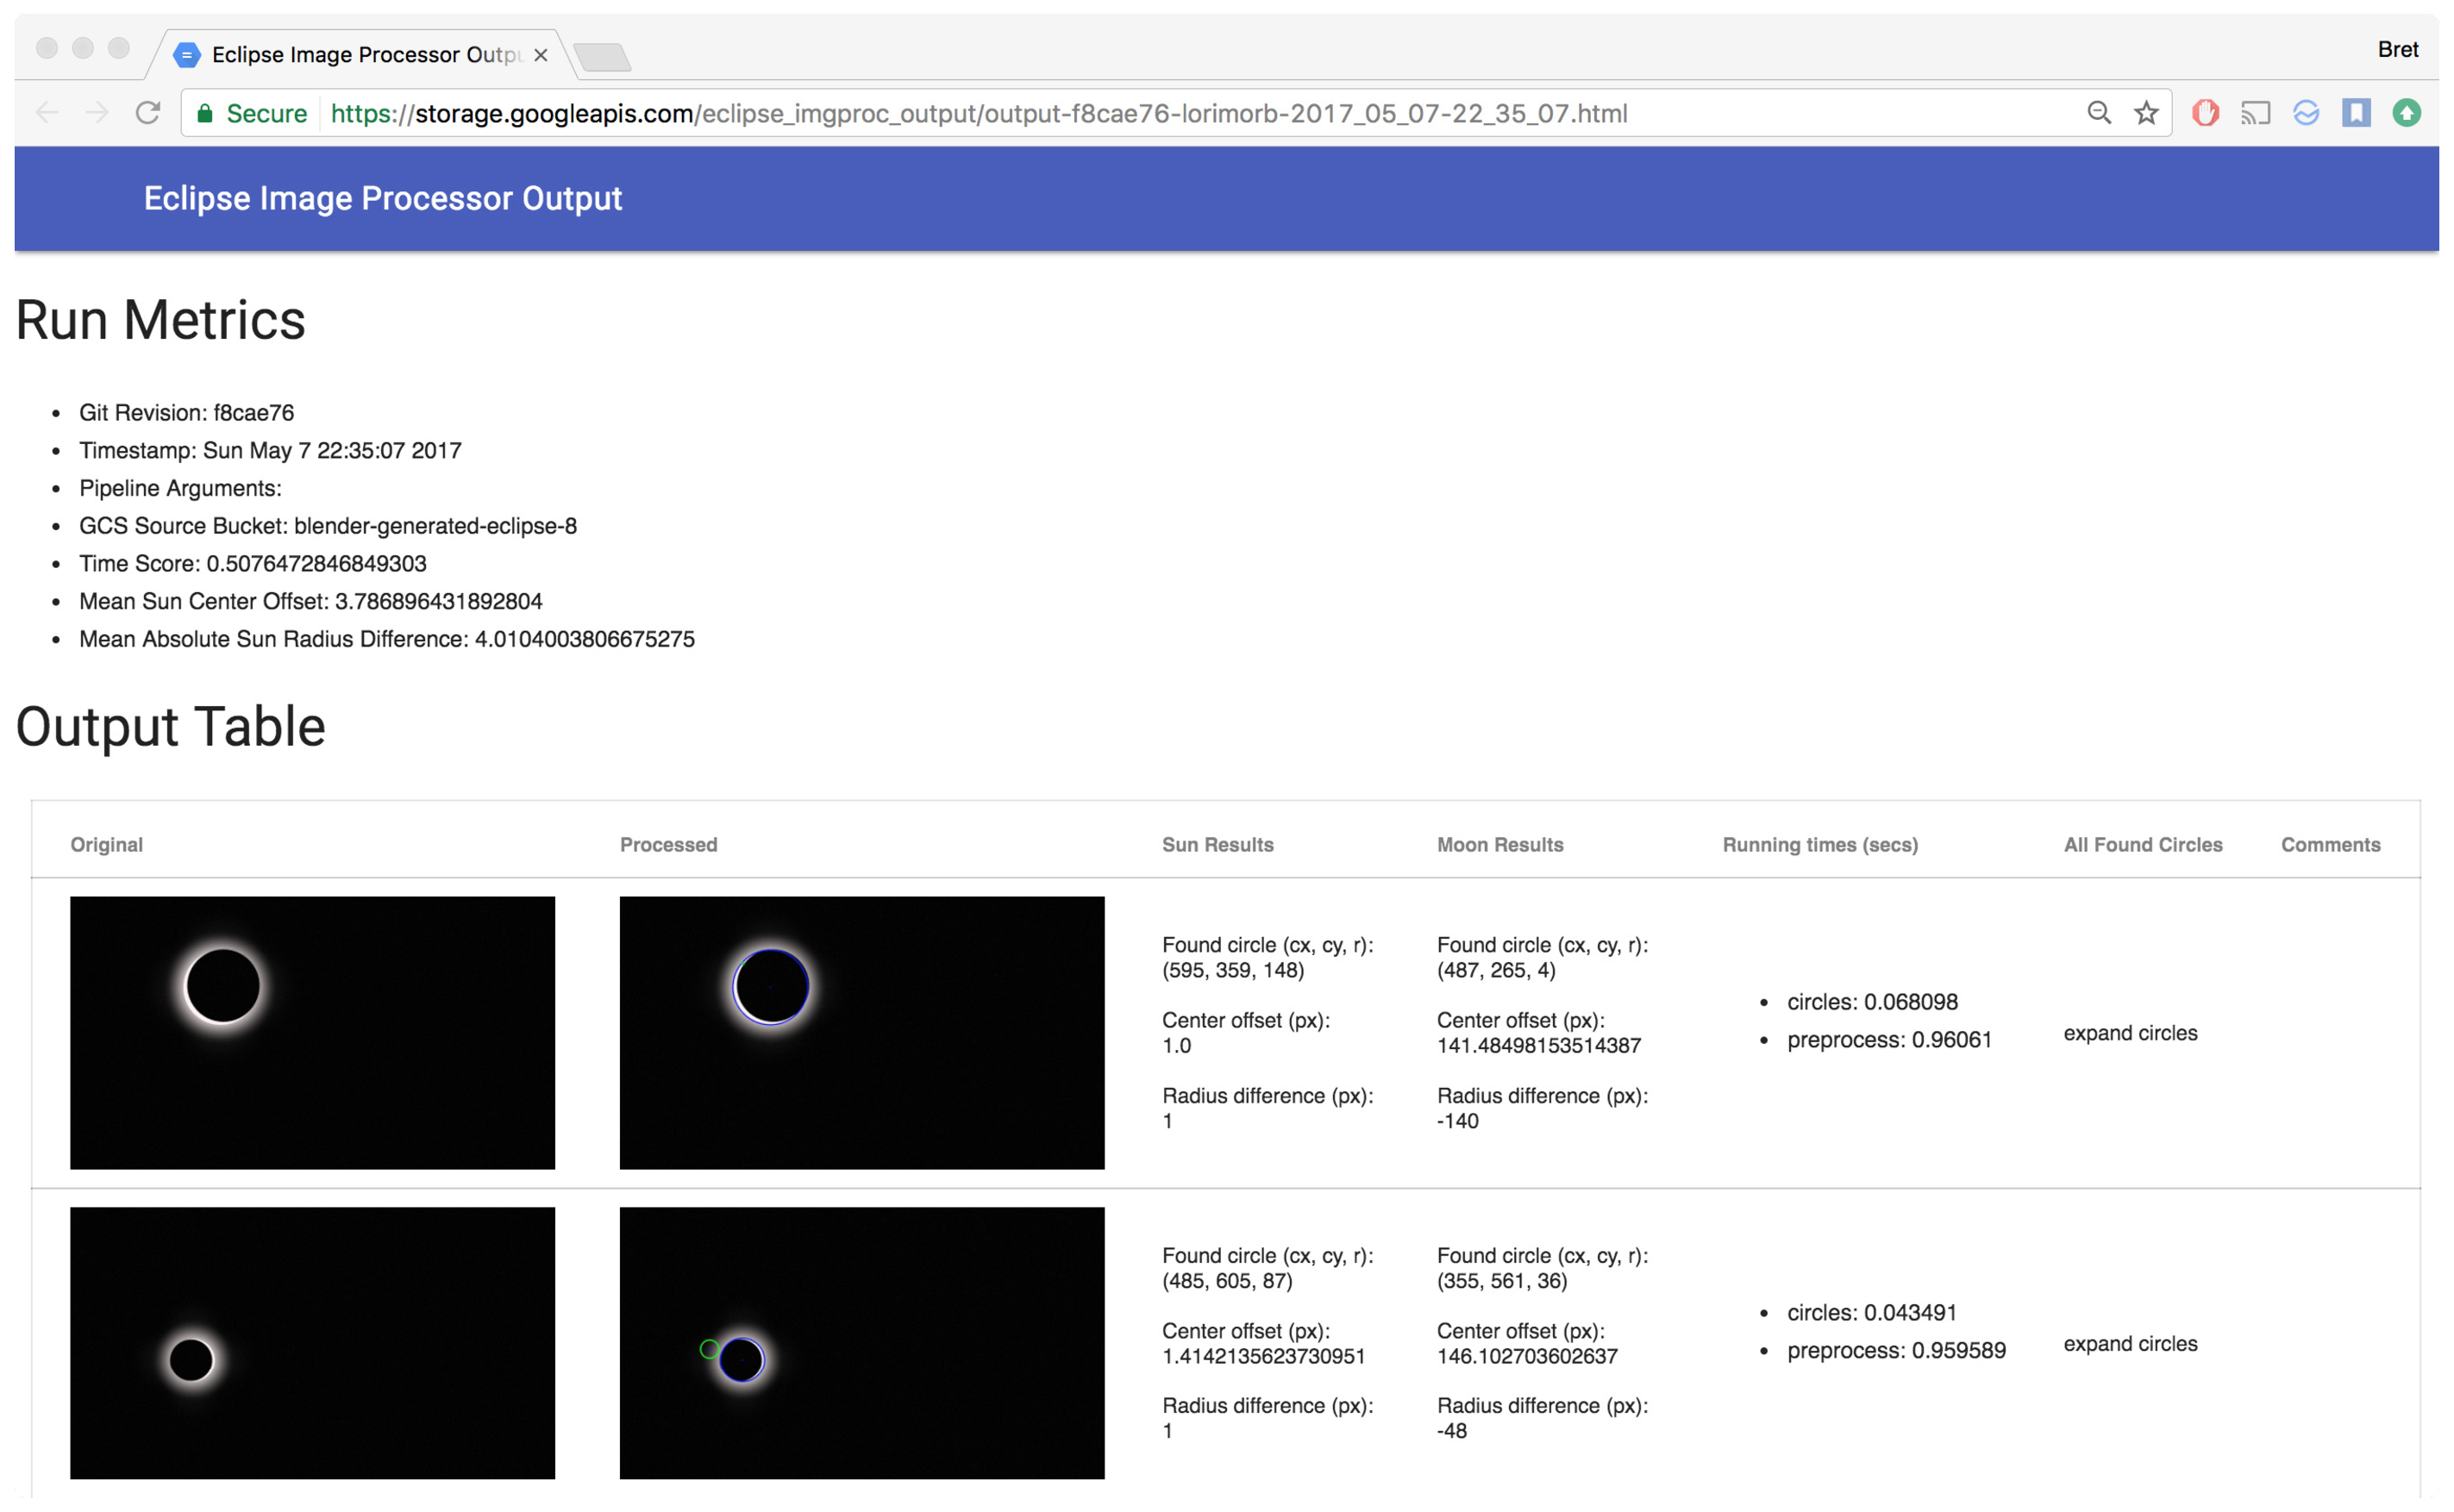
\includegraphics[width=\textwidth]{imgproc.eps}
        \caption{Image Processor Developer Pipeline Results File}
    \end{center}
\end{figure}
\newpage


%%%%%%%%%%%%%%%%%%%%%%%%
%   Weekly Summary     %
%%%%%%%%%%%%%%%%%%%%%%%%
\newpage
\section{Week by Week Summary of Group Activities}

\subsection{Week 1}

    \begin{itemize}

	\item Lorem

    \end{itemize}

\subsection{Week 2}

    \begin{itemize}

	\item Lorem

    \end{itemize}

\subsection{Week 3}

    \begin{itemize}

	\item Lorem

    \end{itemize}

\subsection{Week 4}

    \begin{itemize}

	\item Lorem

    \end{itemize}

\subsection{Week 5}

    \begin{itemize}

	\item Lorem

    \end{itemize}

\subsection{Week 6}

    \begin{itemize}

	\item Lorem

    \end{itemize}

\newpage
\section{Retrospectives}

\begin{table}[!h]
    \centering
    \begin{tabular}{|p{.3\linewidth}|p{.3\linewidth}|p{.3\linewidth}|}

    \cline{3-3}

    \hline \textbf{Positives} & \textbf{Deltas} & \textbf{Actions} \\ \hline

    Lorem & Lorem & Lorem \\ \hline

    \end{tabular}
\end{table}

\end{document}
